\documentclass{beamer}
\usepackage{amsmath,amsbsy,amsopn,amstext,amsfonts,amssymb}
\usepackage{isomath}
\usepackage{ulem}
%\linespread{1.6}  % double spaces lines
\usepackage{graphicx}
\usepackage{subfigure}
\usepackage{color}
\usepackage{optidef}  % define optimization problems
\usepackage{multicol}  % multiple columns
\usepackage{listings} % for python code
\usepackage{mathrsfs}

\usepackage{polynom}
\newcommand{\adj}{\mathrm{adj}}
\newcommand{\constrainedmin}[3]{
		\begin{mini*}|s|
		{#2}{#1}{}{}
		\addConstraint{#3}
		\end{mini*}
}

\newcommand{\rwbcomment}[1]{{\color{blue}RWB:#1}}
\newcommand{\defeq}{\stackrel{\triangle}{=}}
\newcommand{\abs}[1]{\left|#1\right|}
\newcommand{\norm}[1]{\left\|#1\right\|}
\newcommand{\iprod}[1]{\left<#1\right>}
\newcommand{\ellbf}{\boldsymbol{\ell}}
\newcommand{\nubf}{\boldsymbol{\nu}}
\newcommand{\mubf}{\boldsymbol{\mu}}
\newcommand{\abf}{\mathbf{a}}
\newcommand{\bbf}{\mathbf{b}}
\newcommand{\cbf}{\mathbf{c}}
\newcommand{\dbf}{\mathbf{d}}
\newcommand{\ebf}{\mathbf{e}}
\newcommand{\fbf}{\mathbf{f}}
\newcommand{\gbf}{\mathbf{g}}
\newcommand{\hbf}{\mathbf{h}}
\newcommand{\ibf}{\mathbf{i}}
\newcommand{\jbf}{\mathbf{j}}
\newcommand{\kbf}{\mathbf{k}}
\newcommand{\lbf}{\mathbf{l}}
\newcommand{\mbf}{\mathbf{m}}
\newcommand{\nbf}{\mathbf{n}}
\newcommand{\obf}{\mathbf{o}}
\newcommand{\pbf}{\mathbf{p}}
\newcommand{\qbf}{\mathbf{q}}
\newcommand{\rbf}{\mathbf{r}}
\newcommand{\sbf}{\mathbf{s}}
\newcommand{\tbf}{\mathbf{t}}
\newcommand{\ubf}{\mathbf{u}}
\newcommand{\vbf}{\mathbf{v}}
\newcommand{\wbf}{\mathbf{w}}
\newcommand{\xbf}{\mathbf{x}}
\newcommand{\ybf}{\mathbf{y}}
\newcommand{\zbf}{\mathbf{z}}
\newcommand{\Jbf}{\mathbf{J}}
\newcommand{\Acal}{\mathcal{A}}
\newcommand{\Bcal}{\mathcal{B}}
\newcommand{\Lcal}{\mathcal{L}}
\newcommand{\Ncal}{\mathcal{N}}
\newcommand{\Rcal}{\mathcal{R}}
\definecolor{darkolivegreen}{rgb}{0.33, 0.42, 0.18}

\makeatletter
\newenvironment<>{proofstart}[1][\proofname]{%
    \par
    \def\insertproofname{#1\@addpunct{.}}%
    \usebeamertemplate{proof begin}#2}
  {\usebeamertemplate{proof end}}
\newenvironment<>{proofcont}{%
  \setbeamertemplate{proof begin}{\begin{block}{}}
    \par
    \usebeamertemplate{proof begin}}
  {\usebeamertemplate{proof end}}
\newenvironment<>{proofend}{%
    \par
    \pushQED{\qed}
    \setbeamertemplate{proof begin}{\begin{block}{}}
    \usebeamertemplate{proof begin}}
  {\popQED\usebeamertemplate{proof end}}
\makeatother

\title{ECEn 671: Mathematics of Signals and Systems}
\author{Randal W. Beard}
\institute{Brigham Young University}
\date{\today}

\begin{document}

%-------------------------------
\begin{frame}
	\titlepage
\end{frame}

%%%%%%%%%%%%%%%%%%%%%%%%%%%%%%%%%%%%%%%%%%%%%%%%%%%%%%%%%%%%%%%%%
\section{Inequality Constraints: Kuhn-Tucker Conditions}
\frame{\sectionpage}

%----------------------------------
\begin{frame}\frametitle{Inequality Constraints}
	\begin{columns}
		\begin{column}{0.5\textwidth}
			Lets first consider the problem with just inequality constraints, i.e.
			\begin{mini*}|s|
				{}{f(x)}{}{}
				\addConstraint{\gbf(x) \leq 0}
			\end{mini*}
			where $\gbf(x) \leq 0$ means that
			\[
				\begin{pmatrix}
			    	g_1(x)\\
			    	\vdots\\
			    	g_q(x)
			  	\end{pmatrix} 
			  	\leq \begin{pmatrix} 
		 				0 \\ \vdots \\ 0
					 \end{pmatrix}
			\]
			i.e., element-wise.			
		\end{column}
		\begin{column}{0.5\textwidth}
			For example, let $x \in \mathbb{R}^2$ and let $q = 3$.
			\begin{center}
				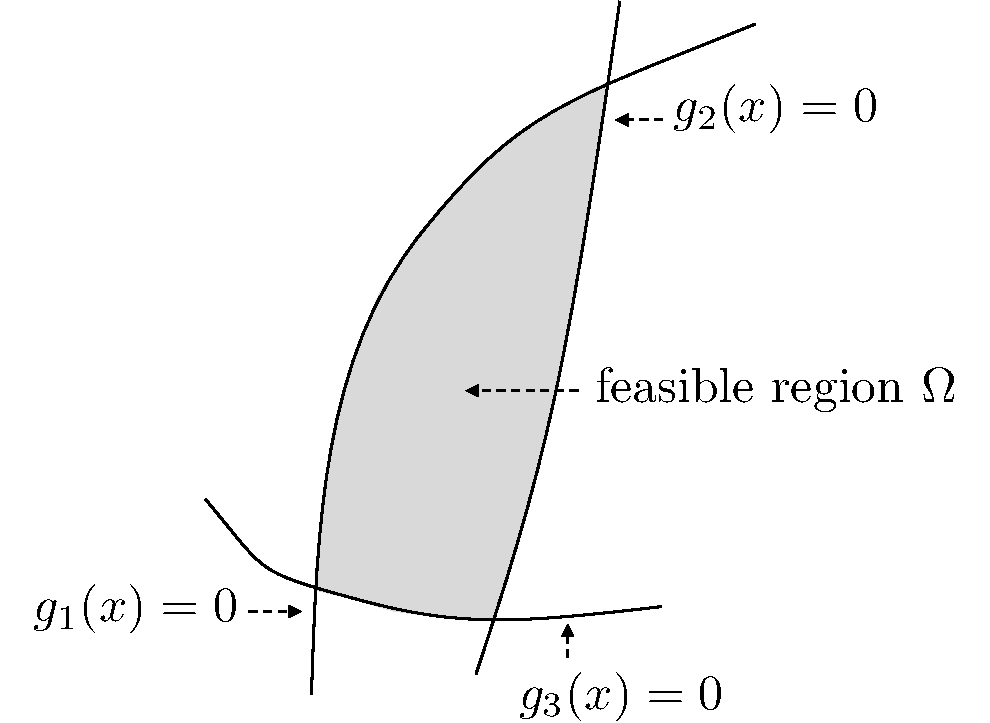
\includegraphics[width=0.99\textwidth]
					{figures/chap18_feasible_region}
			\end{center}			
		\end{column}
	\end{columns}
\end{frame}

%----------------------------------
\begin{frame}\frametitle{Inequality Constraints}
	{\color{blue}Case I.}
	If the local min is in the interior of $\Omega$, then clearly
	\[ 
		\nabla f(x^{\ast}) = 0 
	\]
	or
	\[ 
		\nabla f(x^{\ast}) 
			+ 0 \cdot \nabla g_1(x^{\ast}) 
			+ 0 \cdot \nabla g_2(x^{\ast}) 
			+ 0 \cdot g_3(x^{\ast}) = 0.
	\]
\end{frame}

%----------------------------------
\begin{frame}\frametitle{Inequality Constraints}
	{\color{blue}Case II.}
	The local minimum is on the boundary but not at a corner
	\begin{center}
		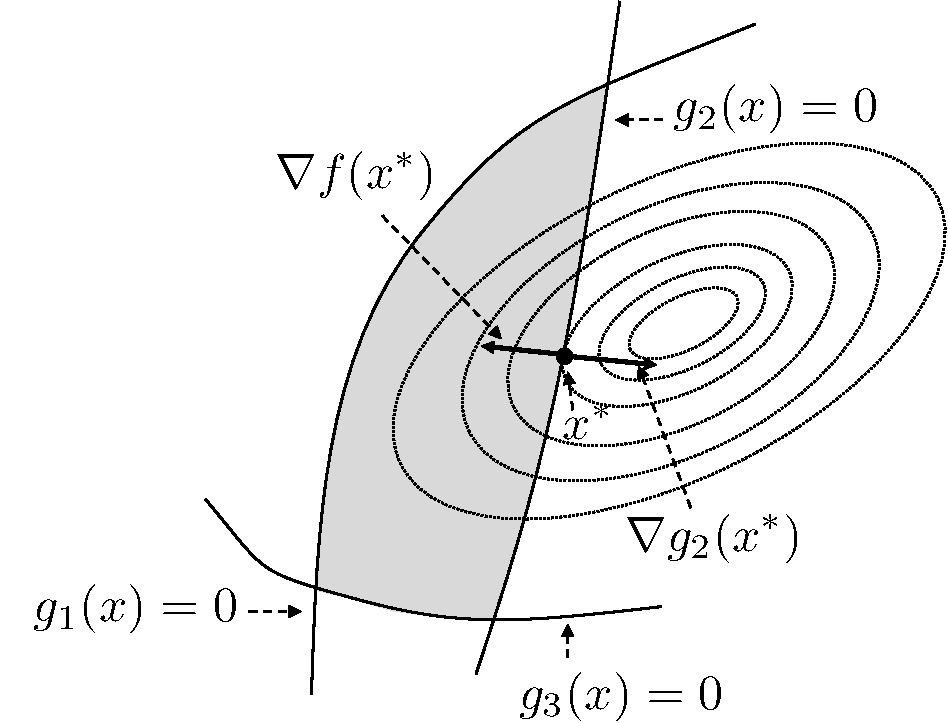
\includegraphics[width=0.5\textwidth]
			{figures/chap18_gradient_of_g}
	\end{center}
	Since in this case $g_1$  is an equality constraint, we must have that $\nabla f(x^{\ast}) \parallel \nabla g_1(x^{\ast})$.  In fact, in this case the two vectors point in opposite directions!  Therefore
	\[
		\nabla f(x^{\ast}) + \mu_1 \nabla g_1(x^{\ast}) + 0\cdot \nabla g_2(x^{\ast}) + 0\cdot g_3 (x^{\ast}) = 0.
	\]	
\end{frame}

%----------------------------------
\begin{frame}\frametitle{Inequality Constraints}
	{\color{blue}Case III.}
		
	\begin{center}
		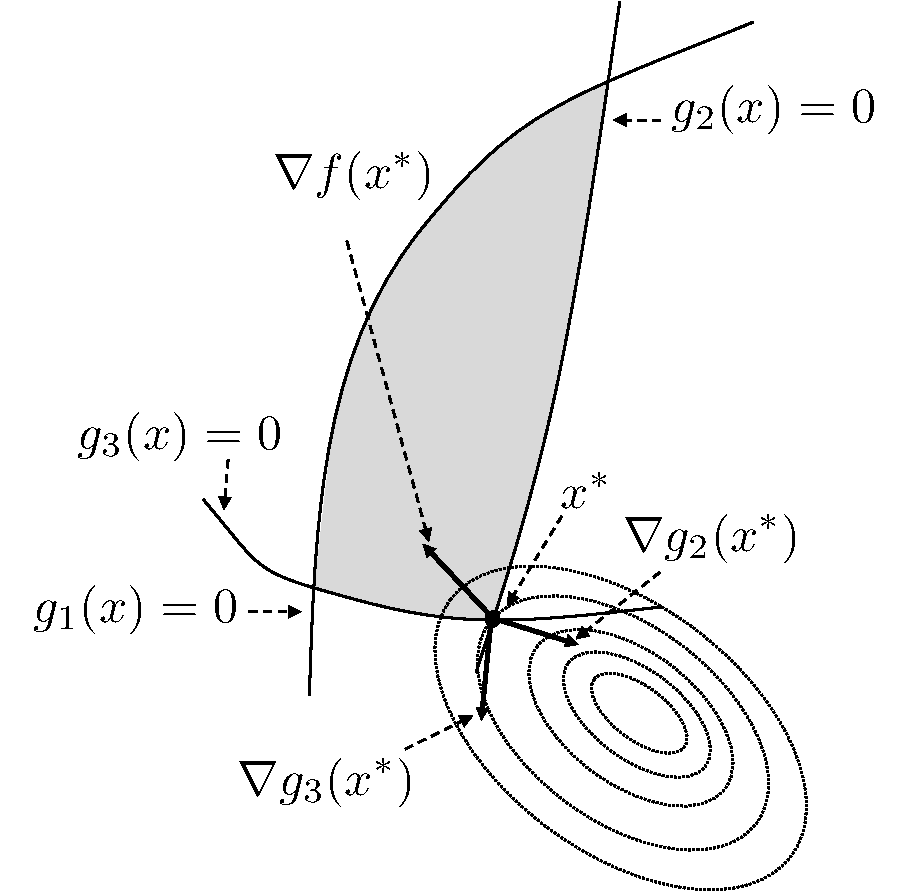
\includegraphics[width=0.5\textwidth]
			{figures/chap18_two_inequality_constraints}
	\end{center}
	In this case, $\nabla f(x^{\ast})$ is in the linear span of $\nabla g_1(x^{\ast})$ and $\nabla g_2(x^{\ast})$ where the coefficients are negative.  Therefore
	\[ 
		\nabla f(x^{\ast}) 
			+ \mu_1 \nabla g_1(x^{\ast}) 
			+ \mu_2 \nabla g_2 (x^{\ast}) 
			+ 0\cdot g_3 (x^{\ast}) = 0 
	\]
	where $\mu_1 > 0$ and $\mu_2 > 0$.
\end{frame}

%----------------------------------
\begin{frame}\frametitle{Inequality Constraints}
	In general, for inequality constraints at a local minimum $x^{\ast}$ we have that
	\begin{enumerate}
	\item $\nabla f(x^{\ast}) + \nabla \gbf(x^{\ast})\mu = 0$
	\item $\gbf(x^{\ast})^\top  \mu = 0$
	\item $\mu \geq 0$
	\end{enumerate}
	
	\vfill

	Conditions (1) and (3) together mean that $\nabla f(x^{\ast})$ is contained in the (negative) linear span of $\{\nabla g_1(x^{\ast}),\ldots,\nabla g_{q}(x^{\ast}) \}$.
	
	\vfill
	
	Condition (2): Note that if the constraint is active, i.e. $g_i(x^{\ast}) = 0$ then $\mu_i$ can be nonzero, but if $g_i$ is inactive, i.e. $g_i(x^{\ast}) < 0$ then $\mu_i$ must be zero to satisfy (2).		
\end{frame}

%----------------------------------
\begin{frame}\frametitle{Inequality Constraints}
	Now lets go back to the general constrained optimization problem:
	\begin{mini*}|s|
		{}{f(x)}{}{}
		\addConstraint{\hbf(x) = 0}
		\addConstraint{\gbf(x) \leq 0}
	\end{mini*}	
	where 
	$f:\mathbb{R}^n\to \mathbb{R}$,
	$h(x):\mathbb{R}^n\to\mathbb{R}^p$,
	$g(x):\mathbb{R}^n\to\mathbb{R}^q$.
	
	\begin{definition}
	$x^{\ast}$ is a \underline{regular point} if $\nabla h_i(x^{\ast}), i = 1, \ldots, p$ and $\nabla g_j(x^{\ast})$ are linearly independent for all $j=1,\dots, q$ such that $g_j(x^{\ast})$ is active.		
	\end{definition}
\end{frame}
	
%----------------------------------
\begin{frame}\frametitle{Inequality Constraints}
	For example, suppose that
	$\hbf = \begin{pmatrix}
	    	h_1\\h_2
	  	 \end{pmatrix}$, and 
	$\gbf = \begin{pmatrix}
	    	g_1\\g_2\\g_3
	  	 \end{pmatrix}$.
	\begin{center}
		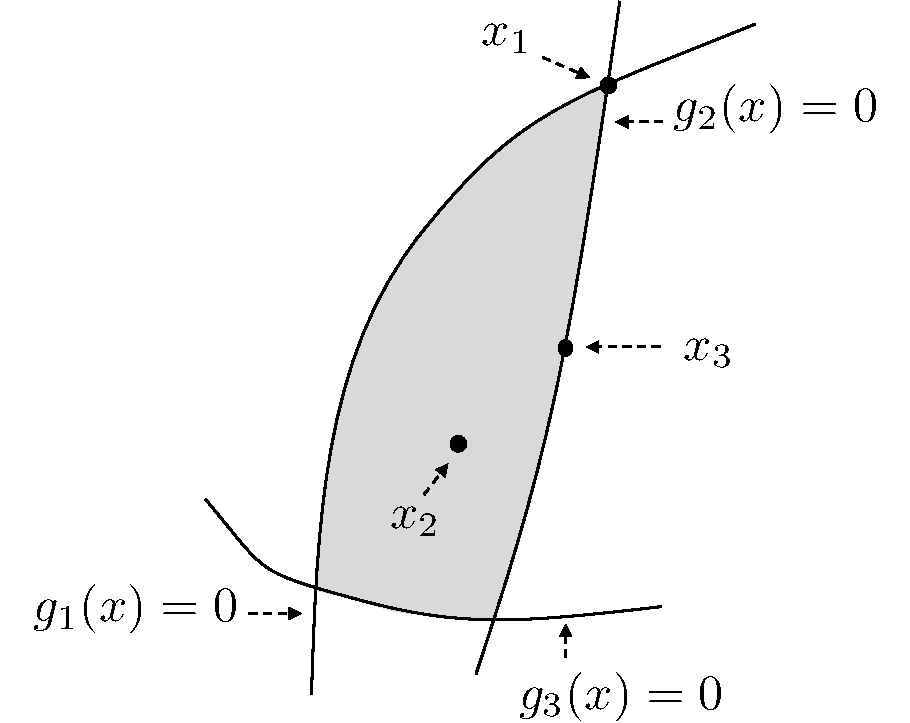
\includegraphics[width=0.4\textwidth]
			{figures/chap18_feasible_points} 
	\end{center}

	  	 
	Then $x^{\ast}$ is a regular point at:
	\begin{itemize}
		\item $x_1$ if 
			$\{ \nabla h_1(x_1), \nabla h_2(x_1), \nabla g_1(x_1), \nabla g_2(x_1) \}$ are  linearly independent.
		\item $x_2$ if 
			$\{ \nabla h_1(x_2), \nabla h_2(x_2) \}$ are linearly independent.
		\item $x_3$ if 
			$\{ \nabla h_1(x_3), \nabla h_2(x_3), \nabla g_1(x_3) \}$ are linearly independent.
	\end{itemize}
\end{frame}

%----------------------------------
\begin{frame}\frametitle{Kuhn Tucker Conditions: Necessary Conditions}	
	\begin{theorem}[Moon Theorem 18.6]
		Let $x^{\ast}$ be a regular local minimum, then 
		$\exists \lambda \in \mathbb{R}^p$ 
		(regular Lagrange multipliers), and
		$\exists \mu \in \mathbb{R}^q$, 
		such that
		\begin{enumerate}
		  \item $\mu \geq 0$ (element wise)
		  \item $\gbf^\top (x^{\ast})\mu = 0$
		  \item $ \nabla f(x^{\ast}) + \nabla \hbf^\top (x^{\ast})\lambda + \nabla \gbf^\top (x^{\ast})\mu = 0$.
		\end{enumerate}		
	\end{theorem}
\end{frame}

%----------------------------------
\begin{frame}\frametitle{Kuhn Tucker Conditions: Sufficient Conditions}	
	\begin{theorem}[Moon 18.7]
		Suppose $f,g,h$ are in $C_2$.
		If there exist $\lambda \in \mathbb{R}^p, \mu \in \mathbb{R}^q$ such that at $x^{\ast}$
		\begin{enumerate}
		  \item $\mu \geq 0$
		  \item $\gbf^\top (x^{\ast})\mu = 0$
		  \item $\nabla f(x^{\ast}) + \nabla \hbf^\top (x^{\ast})\lambda + \nabla \gbf^\top (x^{\ast})\mu = 0$
		  \item $p^\top (\nabla^2f(x^{\ast}) + \sum_{k=1}^p \nabla^2 h_k(x^{\ast})\lambda_k + \sum_{k=1}^q \nabla g_k(x^{\ast})\mu_k )p > 0 $
		\end{enumerate}
		for all $p$ in the tangent plane of the \underline{active} constraints, then $x^{\ast}$ is a local constrained minimum.		
	\end{theorem}
\end{frame}

%----------------------------------
\begin{frame}\frametitle{Kuhn Tucker Conditions: Example 18.9.1}
	\begin{mini*}|s|
		{}{3x_1^2 + 4x_2^2 + 6x_1x_2 - 8x_2 - 6x_1}{}{}
		\addConstraint{x_1^2 + x_2^2 - 9 \leq 0}
		\addConstraint{2x_1 - x_2 - 4 \leq 0}
	\end{mini*}
	The necessary conditions are:
	\begin{align*}
		6x_1 + 6x_2 - 6 + \mu_1(2x_1)+\mu_2(2) &= 0\\
		8x_2 + 6x_1 - 8 + \mu_1(2x_2)+\mu_2(-1) &= 0\\
		\mu_1(x_1^2+x_2^2-9) + \mu_2(2x_1 - x_2 - 4) &= 0 \\
		\mu_1 \geq 0, \mu_2 \geq 0
	\end{align*}
\end{frame}

%----------------------------------
\begin{frame}\frametitle{Kuhn Tucker Conditions: Example 18.9.1}
	Lets try various combinations of active constraints:
	
	\begin{columns}
		\begin{column}{0.5\textwidth}
			\textcolor{blue}{Case I  (Both inactive) 
			i.e. $\mu_1 = \mu_2 \ 0$}
			
			Therefore, must solve
			\begin{align*}
			  6x_1 + 6x_2 - 6 &= 0\\
			  8x_2 + 6x_1 - 8 &= 0\\
			\intertext{i.e.,}\\
			\begin{pmatrix}
			    6 & 6\\
			    6 & 8
			  \end{pmatrix}\begin{pmatrix}
			    x_1\\x_2
			  \end{pmatrix}&=\begin{pmatrix}
			    6\\8
			  \end{pmatrix}\\
			\implies 
			\begin{pmatrix}
			    x_1\\x_2
			  \end{pmatrix}&=\begin{pmatrix}
			    0\\1
			  \end{pmatrix}
			\end{align*}	
		\end{column}
		\begin{column}{0.5\textwidth}
			Check inequality constraints:
			\begin{align*}
				g_1(x) &= 1 - 9 = -8 \leq 0 \\
				g_2(x) &= -1 - 4 \leq 0
			\end{align*}
			Therefore
			\[
				x^{\ast} = \begin{pmatrix}
			    			0\\1
			  			   \end{pmatrix}, 
			  	\mu^{\ast} = \begin{pmatrix}
			    				0\\0
			  			     \end{pmatrix}
			\]
			satisfies necessary conditions.
			
			Sufficient condition:
			\[ 
				\nabla^2 f 
					= \begin{pmatrix}
			    		6 & 6\\
			    		6 & 8
			  		  \end{pmatrix} > 0  
			\]	
			implies local minimum.		
		\end{column}
	\end{columns}
\end{frame}

%----------------------------------
\begin{frame}\frametitle{Kuhn Tucker Conditions: Example }
	\begin{mini*}|s|
		{}{x_1^2 + x_2^2}{}{}
		\addConstraint{x_1 + x_2 + 1 \leq 0}
		\addConstraint{-x_1 + x_2 + 1 \leq 0}
	\end{mini*}

	\begin{center}
		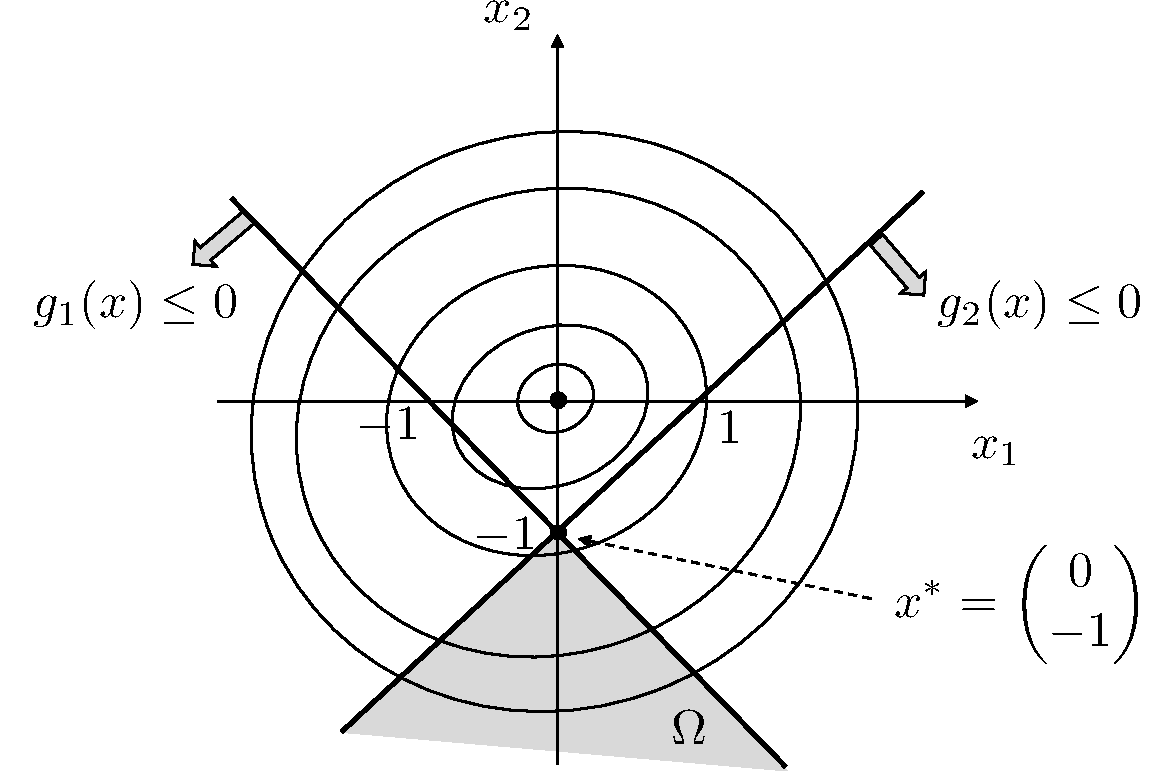
\includegraphics[width=0.5\textwidth]
			{figures/chap18_example2}
	\end{center}
\end{frame}

%----------------------------------
\begin{frame}\frametitle{Kuhn Tucker Conditions: Example }
	The necessary conditions are:
	\begin{align*}
		2x_1 + \mu_1 - \mu_2 &= 0\\
		2x_2 + \mu_1 + \mu_2 &= 0\\
		\mu_1(x_1 + x_2 + 1) + \mu_2(-x_1 + x_2 + 1) &= 0\\
		\mu_1 \geq 0, \mu_2 \geq 0
	\end{align*}	
	Try various combinations of active constraints
	\textcolor{blue}{Case 1: (Both inactive) }
	\begin{align*}
		2x_1 &= 0\\
		2x_2 &= 0
	\end{align*}
	\[ \implies x^{\ast} = \begin{pmatrix}
	    0\\0
	  \end{pmatrix}
	\]
	However, both constraints are violated since
	\begin{align*}
		g_1^{\ast}(x^{\ast}) = 1 \geq 0\\
		g_2(x^{\ast}) = 1 \geq 0.
	\end{align*}
\end{frame}
	
%----------------------------------
\begin{frame}\frametitle{Kuhn Tucker Conditions: Example }
	\textcolor{blue}{Case 2: $g_1$-active, $g_2$-inactive}
	\begin{align*}
		2x_1 + \mu_1 &= 0 \quad\implies x_1 = -\frac{1}{2}\mu_1 \\
		2x_2 + \mu_1 &= 0 \quad\implies x_2 = -\frac{1}{2}\mu_1\\
		\mu_1(x_1 + x_2 + 1) &= 0\\
		\mu_1 > 0
	\end{align*}
	Last two equations imply that
	\[ 
	\mu_1(-\frac{1}{2}\mu_1-\frac{1}{2}\mu_1 + 1) = -\mu_1^2 + \mu_1 = \mu_1(1-\mu_1) = 0.
	\]
	Solving for $\mu_1$ gives $\mu_1 = 0$ or \fbox{$\mu_1 = 1$}.
	Therefore 
	\[
		x^{\ast} = 
			\begin{pmatrix}
	    		-\frac{1}{2} \\
	    		-\frac{1}{2}
	  		\end{pmatrix}
	\]	
\end{frame}

%----------------------------------
\begin{frame}\frametitle{Kuhn Tucker Conditions: Example }
	Checking constraints:
	\begin{align*}
		g_1(x^{\ast}) &= -\frac{1}{2} -\frac{1}{2} + 1 = 0 \leq 0 \qquad \text{ ok }\\
		g_2(x^{\ast}) &= \frac{1}{2} -\frac{1}{2} + 1 = 1 \geq 0 \qquad \text{ no }
	\end{align*}	
	\textcolor{blue}{Case 3: $g_1$-inactive, $g_2$-active}
	 Similar results to Case 2.
	 
	 \vfill

	\textcolor{blue}{Case 4: Both active}
	\begin{align*}
		& \mu_1(\frac{1}{2}\mu_2 - \frac{1}{2}\mu_1 - \frac{1}{2}\mu_2-\frac{1}{2}\mu_1 + 1) \\
		& \quad 
		+ \mu_2(-\frac{1}{2}\mu_2 + \frac{1}{2}\mu_1 - \frac{1}{2}\mu_1 - \frac{1}{2}\mu_2 + 1) = 0 \\
		\implies & \mu_1(1-\mu_1) + \mu_2(1-\mu_2) = 0
	\end{align*}	
\end{frame}
	
%----------------------------------
\begin{frame}\frametitle{Kuhn Tucker Conditions: Example }
	A positive solution is
	\[ 
		\begin{pmatrix}
	    	\mu_1\\
	    	\mu_2
	  	\end{pmatrix} = 
	  	\begin{pmatrix}
	    	1\\1
	  	\end{pmatrix} > 0 
	\]
	which gives
	\[
		x^{\ast} = 
			\begin{pmatrix}
	      		0 \\ -1
	    	\end{pmatrix}
	\]
	
	\vfill
	
	Constraints can be verified to be satisfied.
	
	\vfill
	
	
	Sufficient condition:
	\[ 
		\nabla^2 f + \nabla^2 g \mu = 
			\begin{pmatrix}
	    		2 & 0\\
	    		0 & 2
	  		\end{pmatrix} + 
	  		\begin{pmatrix}
	    		0 & 0\\
	    		0 & 0
	  		\end{pmatrix}1 + 
	  		\begin{pmatrix}
	    		0 & 0\\
	    		0 & 0
	  		\end{pmatrix}1 = 
	  		\begin{pmatrix}
	    		2 & 0\\
	    		0 & 2
	  		\end{pmatrix} > 0
	\]
	Therefore $x^{\ast}$ is a local minimum.	
\end{frame}



\end{document}